\documentclass[a4paper,12pt,openright,twoside]{book}

% libreria per scrivere in italiano
\usepackage[italian]{babel}

% libreria per accettare i caratteri utf-8
\usepackage[utf8]{inputenc}

% libreria per impostare il documento
\usepackage{fancyhdr}
\renewcommand{\chaptermark}[1]{\markboth{\thechapter.\ #1}{}}
\renewcommand{\sectionmark}[1]{\markright{\thesection \ #1}{}}
\rhead[\fancyplain{}{\bfseries\leftmark}]{\fancyplain{}{\bfseries\thepage}}
\cfoot{}

% per i collegamenti ipertestuali
\usepackage{hyperref}
\hypersetup{
	colorlinks=true,
	linkcolor=blue,
	citecolor=blue,
	filecolor=blue,
	urlcolor=blue
}

% per le immagini
\usepackage{graphicx}



% documento
\begin{document}

\begin{list}{}{
  \setlength{\topsep}{20pt}
  \setlength{\leftmargin}{-40pt}%
  \setlength{\rightmargin}{-80pt}%
  \setlength{\listparindent}{0pt}%
  \setlength{\itemindent}{0pt}%
  \setlength{\parsep}{0pt}%
 }%
\item[]
\thispagestyle{empty}

\begin{center}
{{\center \fontsize{17.4}{60}\selectfont \textsc{Alma Mater Studiorum $\cdot$ Università di Bologna}}}
\noindent\makebox[\linewidth]{\rule[0.1cm]{15.8cm}{0.1mm}}
\noindent\makebox[\linewidth]{\rule[0.5cm]{15.8cm}{0.6mm}}
{\small{\bf Dipartimento di Informatica - Scienza e Ingegneria (DISI)\\
Corso di Laurea Magistrale in Informatica}}

\end{center}
\vspace{40mm}
\begin{center}
{\LARGE{\bf Collaborative Robbies}}\\
%\vspace{3mm} {\large{\bf Remember when and thing won't be a problem anymore!}}\\
\vspace{3mm} {\large{\bf Relazione di FSC}}
\end{center}
\vspace{20mm}
\begin{center}
{\large{\bf 18 dicembre 2015}}
\end{center}
\vspace{50mm}
\par
\noindent
\begin{minipage}[t]{0.54\textwidth}\raggedright
{\large{\bf Giulio Biagini\\
0000705715\\
giulio.biagini@studio.unibo.it\vspace{\baselineskip}}}\\
\end{minipage}
\hfill
\begin{minipage}[t]{0.54\textwidth}\raggedleft
{\large{\bf Daniele Baschieri\\
0000688992\\
daniele.baschieri@studio.unibo.it}}
\end{minipage}

\end{list}

\clearpage
\newpage
\tableofcontents
\chapter{Introduzione}
In questo capitolo andremo a descrivere \textit{Robby: The Soda-Can-Collecting
Robot}~\cite{biblio:robby}, il progetto a cui questo lavoro si ispira,
riportando alcuni cenni teorici di Intelligenza Artificiale che useremo per
descrivere in maniera più formale la struttura dell'intero progetto.



\section{Robby: The Soda-Can-Collecting Robot}
Robby è un robot il cui compito consiste nel muoversi in uno spazio sporco e
cercare di ripulirlo. Lo spazio può essere visto in modo astratto come una
griglia suddivisa in celle. Robby possiede solamente una vista parziale dello
spazio nel quale si trova: è in grado di vedere cosa è presente nella cella a
nord, in quella a sinistra, nella casella in cui si trova, in quella a destra ed
in quella a sud rispetto alla propria posizione. Le celle possono essere
``pulite'' (vuote), ``sporche'' (nelle quali è presente una lattina da
raccogliere) oppure rappresentare un ostacolo (un muro).\newline
Robby attua un'azione in base alla vista che ha in quel momento dell'ambiente.
Se, ad esempio, vede una lattina nella cella a nord, un muro nella cella a
sinistra e niente nella cella da lui occupata, in quella a destra e nella cella
a sud, questo non si muoverà negli spazi vuoti, né tantomeno sbatterà contro il
muro muovendosi a sinistra, ma si muoverà di un passo verso l'alto, in direzione
della lattina, per poi raccoglierla. Le azioni che Robby può effettuare sono: la
mossa verso nord, verso sinistra, verso destra e verso sud, può decidere di
rimanere fermo, raccogliere una lattina oppure effettuare una mossa casuale
scelta fra le precedenti. Tutte le mosse hanno l'effetto immaginato a parte la
raccolta della lattina. Questa toglierà la lattina dalla mappa nella cella in
cui il robot si trova, se presente, altrimenti lascerà l'ambiente
invariato.\newline
Inizialmente Robby possiede un dna casuale, ovvero, ad ogni vista è associata
un'azione casuale. Robby è però in grado di apprendere come muoversi
correttamente nell'ambiente e come raccogliere lattine. La sua evoluzione è
infatti guidata da un Algoritmo Genetico.



\section{Entità Intelligenti}
Lo scopo dell'\textit{Intelligenza Artificiale} è quello di cercare di capire
come le \textit{entità intelligenti} funzionano ed, in particolare, quello di
cercare di costruire, creare, entità intelligenti.\newline
Negli anni sono state date varie definizioni di entità intelligenti: alcune
fanno paragoni con gli esseri umani, altre usano il principio della razionalità,
alcune definiscono queste entità in base a come pensano, altre a come agiscono.
Nel nostro particolare caso, andremo a definire un'entità come intelligente se
\textit{agisce in modo razionale}, ovvero se ``fa la cosa giusta''.\newline
Affinché \textbf{Robby}, l'entità intelligente che abbiamo il compito di
creare, possa essere definita intelligente, dovrà quindi ``fare la cosa
giusta''. Intuitivamente, siccome il compito del robot sarà quello di muoversi
in uno spazio cercando di pulirlo, ``fare la cosa giusta'' significherà, ad
esempio, non sbattere contro i muri durante il proprio movimento, raccogliere le
lattine durante il proprio passaggio e non tentare di raccogliere lattine dove
queste non sono presenti.



\section{Agenti Intelligenti}
Un \textit{agente intelligente} è un'entità intelligente in grado di percepire
l'ambiente tramite dei \textit{sensori} e compiere delle azioni tramite degli
\textit{attuatori}.\newline
Un agente ha delle \textit{percezioni} dell'ambiente, ovvero l'insieme di tutti
gli input percettivi che provengono dai propri sensori in un dato
istante.\newline
Il comportamento di un agente intelligente è descritto matematicamente da una
\textit{funzione agente}, ovvero l'insieme di tutte le sequenze percettive
e da tutte le relative azioni. L'implementazione di una funzione agente prende
il nome di \textit{programma agente}.\newline
Analizzando la definizione di agente intelligente, possiamo notare come
\textbf{Robby} sia un'entità che appartenga a questa categoria: esso infatti
è in grado di percepire l'ambiente tramite dei sensori che gli permettono di
vedere il contenuto delle celle che lo circondano e possiede degli attuatori che
gli consentono di muoversi e raccogliere lattine.\newline
L'insieme di tutte le viste (percezioni) che Robby può avere dell'ambiente e le
rispettive azioni sono descritte da una funzione agente. Il nostro compito sarà
quello di fornirne un'implementazione attraverso la scrittura di un programma
agente.



\section{Agenti Razionali}
Il nostro obiettivo, però, non è semplicemente quello di creare agenti
intelligenti, ovvero entità in grado di percepire l'ambiente e compiere azioni,
ma, piuttosto, creare \textit{agenti razionali}, ovvero entità sì intelligenti,
ma che ``facciano la cosa giusta''. Questo significa che il programma agente,
per ogni sequenza percettiva, produce un'azione che va a massimizzare una
determinata \textit{misura di prestazione}: se le azioni attuate dall'agente
portano l'ambiente ad attraversare una sequenza di stati che può essere definita
``desiderabile'', allora la misura di prestazione è massimizzata.\newline
Nel caso di \textbf{Robby}, la misura di prestazione da massimizzare sarà sia il
numero di lattine che debbono essere raccolte in un dato ambiente, sia il numero
di passi impiegato per raccoglierle.



\section{Agenti Reattivi Semplici}
Esistono varie tipologie di programmi agente in base alle tipologie di agenti
di cui questi hanno il compito di descrivere il comportamento. I più semplici di
tutti sono gli \textit{Agenti Reattivi Semplici}, ovvero agenti che basano le
proprie azioni solamente sulla percezione corrente. Questi agenti, dunque,
analizzano tutti gli input percettivi che provengono dai sensori in un dato
istante e computano quale azione compiere.\newline
\textbf{Robby} è un agente reattivo semplice in quanto la scelta dell'azione da
attuare è guidata solamente dalla vista che ha in quel momento dell'ambiente.



\section{Agenti in Grado di Apprendere}
Esistono particolari tipologie di agenti che possono essere programmati in modo
che siano \textit{in grado di apprendere}.\newline
Un agente, infatti, può calcolare la scelta delle proprie azioni basandosi su
conoscenze pregresse che ha dell'ambiente, che sono ad esempio state inserite a
priori da un programmatore: in questo caso si dice che l'agente manca di
autonomia. Al contrario un \textit{agente autonomo} è in grado di apprendere
per compensare la presenza di conoscenza parziale o erronea. Un agente in grado
di apprendere ha il vantaggio di poter operare in ambienti all'inizio
sconosciuti, diventando col tempo via via più competente.\newline
Questa tipologia di agenti possiedono, oltre ad un \textit{elemento esecutivo},
che gli permette di selezionare le azioni da compiere, anche un \textit{elemento
di apprendimento}, responsabile del miglioramento interno, il quale usa le
informazioni provenienti dall'\textit{elemento critico} riguardo le
prestazioni correnti dell'agente e determina se e come modificare l'elemento
esecutivo affinché in futuro si comporti meglio. Infine, le entità in grado di
apprendere possiedono un \textit{generatore di problemi}, il cui scopo è quello
di suggerire azioni che portino ad esperienze nuove e significative dalle quali
apprendere.\newline
Nel caso di \textbf{Robby}, quello che vogliamo è un agente autonomo in grado
di apprendere, ovvero un agente che non si basi su conoscenza pregressa da noi
inserita. Per fare questo ci appoggeremo sugli \textit{Algoritmi Genetici}.

\chapter{Obiettivi}
In questo capitolo sono descritti gli obiettivi di questo lavoro. In
particolare, quello che ci interessa non è tanto re-implementare il lavoro
proposto da Melanie Mitchell~\cite{biblio:robby}, quanto piuttosto realizzare un
sistema che ci permetta di studiare come, inserendo più entità nell'ambiente,
queste si influenzino a vicenda.\newline
Lo scopo principale, dunque, è analizzare se può esservi \textbf{collaborazione
spontanea} o meno fra le entità che si trovano a nella stessa mappa.

\section{Entità Invisibili - Vista a Croce}
Come prima cosa andremo a cercare di stabilire quali sono le performance di due
agenti che si muovono sulla mappa senza vedersi, ovvero ignorando la posizione
dell'altro robot. Sarà dunque ammesso trovarsi nella stessa cella e raccogliere
la stessa lattina.\newline
I due robot avranno vista a croce, ovvero come quella descritta nel capitolo
introduttivo: potranno vedere la casella a nord, quella a sinistra, quella nella
quale si trovano, quella a destra e quella a sud.\newline
I risultati ottenuti saranno poi usati come ``caso base'', per fare un confronto
con le simulazioni lanciate successivamente.

\section{Entità Invisibili - Vista Quadrata}
In questo secondo test, così come nel caso precedente, le due entità non saranno
in grado di vedersi ma avranno una percezione maggiore della mappa nella quale
si troveranno. Potranno infatti vedere uno spazio di 3x3 celle dove il robot
occupa la posizione centrale (seconda riga e seconda colonna).\newline
Questa prova ci permetterà di capire se potendo vedere una porzione di mappa
maggiore, i robot saranno avvantaggiati nella pulizia della stessa, ovvero, se
disponendo di più risorse (sensori più potenti) saranno in grado di massimizzare
maggiormente la misura di prestazione: sia essa la raccolta di un numero
maggiore di lattine, sia essa la raccolta dello stesso numero di lattine ma con
un numero minore di passi.

\section{Entità Visibili - Vista a Croce}
Con quest'ultima simulazione vedremo cosa succede dando la possibilità ai due
robot di vedersi. In questo caso non sarà tollerata la compresenza nella
medesima cella.\newline
Vedremo così se i due robot impareranno a collaborare o se invece la presenza
di uno ostacolerà l'altro.

\chapter{Progettazione}
In questo capitolo parleremo di come è stato implementato l'algrotimo genetico
che ha permesso l'apprendimento di una strategia di pulizia alle coppie che
saranno impegnate sulla mappa.

\section{Algoritmi Genetici: schema generale}
Gli \textit{Algoritmi Genetici} sono algoritmi spesso usati in tutte quelle
situazioni nelle quali risulta difficile andare a progettare una determinata
strategia che ci permetta di arrivare ad una soluzione. Questi algoritmi sono
difatti usati per far sì che siano loro stessi ad evolvere il sistema in modo
che esso arrivi autonomamente ad una soluzione. Uno dei campi nei quali sono
maggiormente impiegati, infatti, sono i \textit{Sistemi Complessi}.\newline
Per far sì che \textbf{Robby} possa muoversi e pulire l'ambiente raccogliendo il
maggior numero di lattine con il minor numero di mosse, non conoscendo a priori
la posizione del robot stesso nella mappa, né delle lattine, non rimane che
progettare un algoritmo genetico che permetta ai robot di apprendere una buona
strategia.\newline
La struttura utilizzata nel paper di riferimento~\cite{biblio:robby} è la
seguente:
\begin{itemize}
	\item dapprima sono generati \textit{POPULATION\_SIZE} individui con un dna
	casuale, ovvero, ad ogni possibile vista è associata una mossa scelta a caso
	fra quelle possibili;
	\item dopodiché, per \textit{NUM\_GENERATIONS}:
	\begin{itemize}
		\item viene calcolato il \textit{valore di fitness} per ogni individuo
		assegnando un punteggio 10 nel caso in cui un robot raccolga una
		lattina, -1 se il robot tenta di raccogliere una lattina in una cella
		dove questa non sia presente e -5 punti se il robot tenta di muoversi in
		una casella occupata da un ostacolo (muro). Questa operazione viene
		effettuata per \textit{NUM\_ACTIONS\_PER\_SESSIONS} passi e ripetuta per
		\textit{SESSIONS\_NUMBER} diverse sessioni. Ogni sessione prevede la
		generazione di una mappa nella quale le lattine sono posizionate
		casualmente nelle celle (ogni cella ha la medesima probabilità di
		ospitarne una) così come la posizione del robot è scelta casualmente.
		La mappa ha dimensione 10x10 con 10 lattine. Alla fine, ogni robot
		ottiene un valore di fitness mediato sul numero di sessioni. Il numero
		di azioni su ogni mappa è fissato a 200, così come il numero di
		sessioni;
		\item si procede poi ordinando gli individui in base al proprio valore
		di fitness;
		\item sono scelti due individui nella popolazione con una probabilità
		che varia linearmente in base all'ordinamento (l'individuo con il
		maggiore valore di fitness avrà probabilità più alta di essere scelto
		rispetto al secondo e così via\dots) e viene applicato il
		\textit{crossover}. Questo procedimento genererà due nuovi figli ed è
		ripetuto fino alla generazione della nuova popolazione;
		\item una volta ottenuta la nuova generazione, ogni gene (azione
		corrispondente ad una vista) può essere mutato con una probabilità pari
		a \textit{MUTATION\_PROBABILITY}: 0.5\%.
	\end{itemize}
\end{itemize}

\section{Collaborazione}
Siccome il nostro obiettivo è quello di studiare la collaborazione fra più
robot, nella mappa saranno presenti contemporaneamente 2 agenti. Questo farà sì
che la grandezza POPULATION\_SIZE non indichi il numero di robot nellpopolazione ma il numero di coppie. Dunque, il numero di entità sarà pari al
popolazione ma il numero di coppie. Dunque, il numero di entità sarà pari al
doppio.

\section{Funzione di Fitness}
La presenza di due robot nella mappa comporta anche la modifica dei come la
funzione di fitness valuta gli individui. Il valore di fitness non riguarderà un
singolo agente, ma la coppia.\newline
Nel caso in cui i due robot abbiano la possibilità di vedersi, poi, sarà
assegnato un valore negativo di -5 punti anche nel caso le due entità cerchino
di occupare la stessa cella, scontrandosi, così come avviene nel caso in cui un
robot tenti di muoversi contro il muro. Nel caso in cui non si vedono ed
entrambi occupano la stessa cella nella quale è presente una lattina e cercano
di raccoglierla, il secondo robot non prenderà punteggio negativo in quanto la
lattina è già stata raccolta dal primo. Non si avrà però neanche l'incremento
del valore di fitness di 20 punti (10 per l'azione di raccolta del primo e 10
per l'azione di raccolta del secondo). In un caso simile sarà incrementato il
valore di fitness di soli 10 punti in quanto entrambi hanno fatto l'azione
corretta ma solo una lattina è stata raccolta.

\section{Selezione dei Genitori}
La tecnica da noi usata per generare la nuova popolazione non è esattamente
quella descritta nel paper. Difatti, a seconda delle varie simulazioni, saranno
copiati alcuni individui dalla vecchia alla nuova generazione senza passare
tramite il crossover.

\section{Crossover}
La tecnica di crossover da noi usata è quella descritta nel paper, ovvero: è
scelto un punto di taglio casuale nel dna dei due genitori per generare i figli.
Avendo però delle coppie la strategia cambia lievemente: sono scelte due coppie
come genitori dove, il primo Robby della prima coppia ed il primo Robby della
seconda generano il primo figlio, mentre il secondo Robby della prima coppia ed
il secondo della seconda coppia generano il secondo figlio. Per ognuno dei due
figli, il punto di taglio nel dna dei genitori varia.

\section{Mutazione Genetica}
La mutazione genetica è fatta nella maniera standard, mutando i geni dei due
robot generati in accordo con una percentuale fissata. Anche nel caso in cui
siano copiati degli individui dalla vecchia alla nuova generazione (senza dunque
l'uso del crossover), questi subiranno mutazioni.

\chapter{Implementazione}
TODO

\section{ANSI C}
TODO

\section{MPI}
TODO -> parlare dei seed

\chapter{Risultati}
In questo capitolo saranno presentati i risultati ottenuti nelle varie
simulazioni. Quando non meglio specificato, i parametri sono stati mantenuti
come quelli indicati nel paper. Visto il nostro assegnamento dei valori di
fitness, il punteggio massimo è 100 punti, ottenuto non entrando mai nei muri,
non scontrandosi mai con altri robot e raccogliendo tutte le lattine.

\section{Entità Invisibili - Vista a Croce}
\begin{figure}[ht]
	\centering
	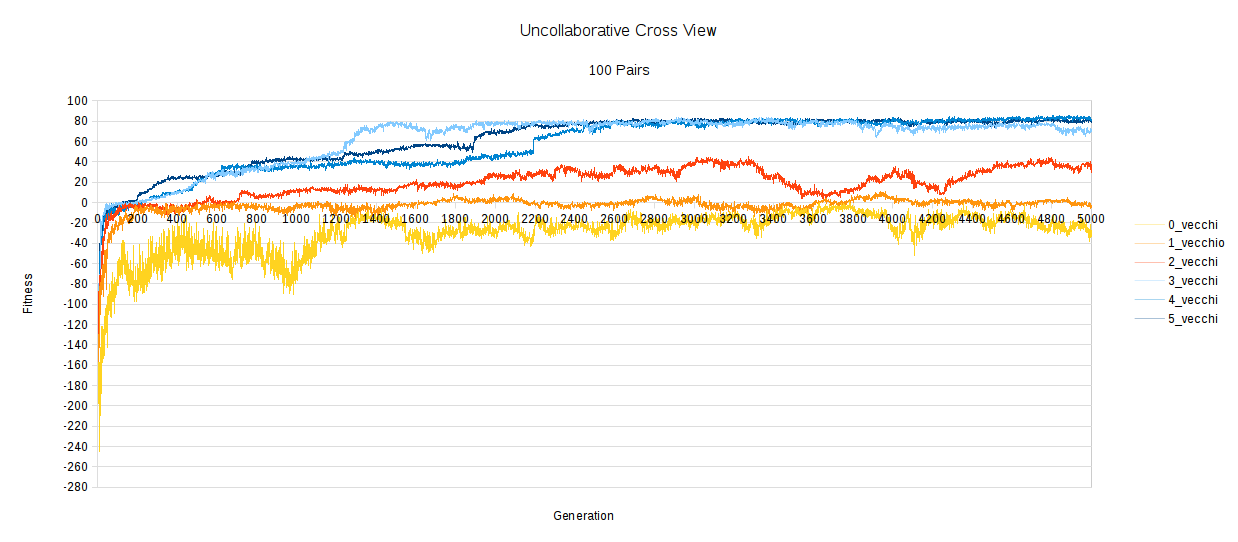
\includegraphics[scale=0.7,angle=90]{imgs/uncollaborative_cross_100_pairs_0_5_vecchi.png}
	\caption{Vista a croce non collaborativa, 100 coppie}
	\label{figure:uncoll_cross_100_0_5}
\end{figure}
\begin{figure}[ht]
	\centering
	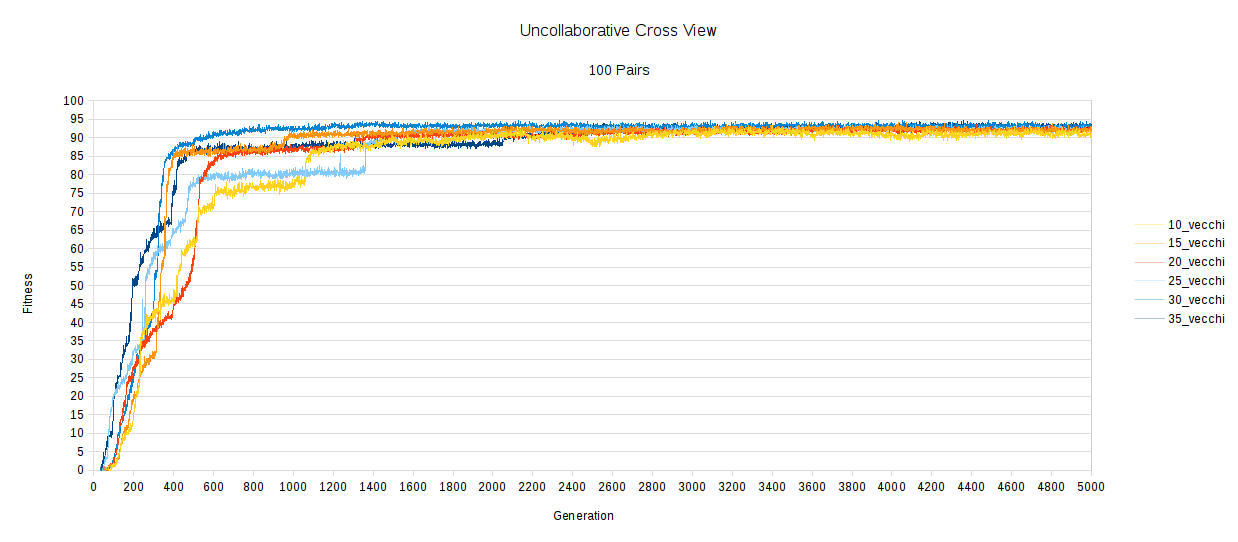
\includegraphics[scale=0.7,angle=90]{imgs/uncollaborative_cross_100_pairs_10_35_vecchi.png}
	\caption{Vista a croce non collaborativa, 100 coppie}
	\label{figure:uncoll_cross_100_10_35}
\end{figure}
\begin{figure}[ht]
	\centering
	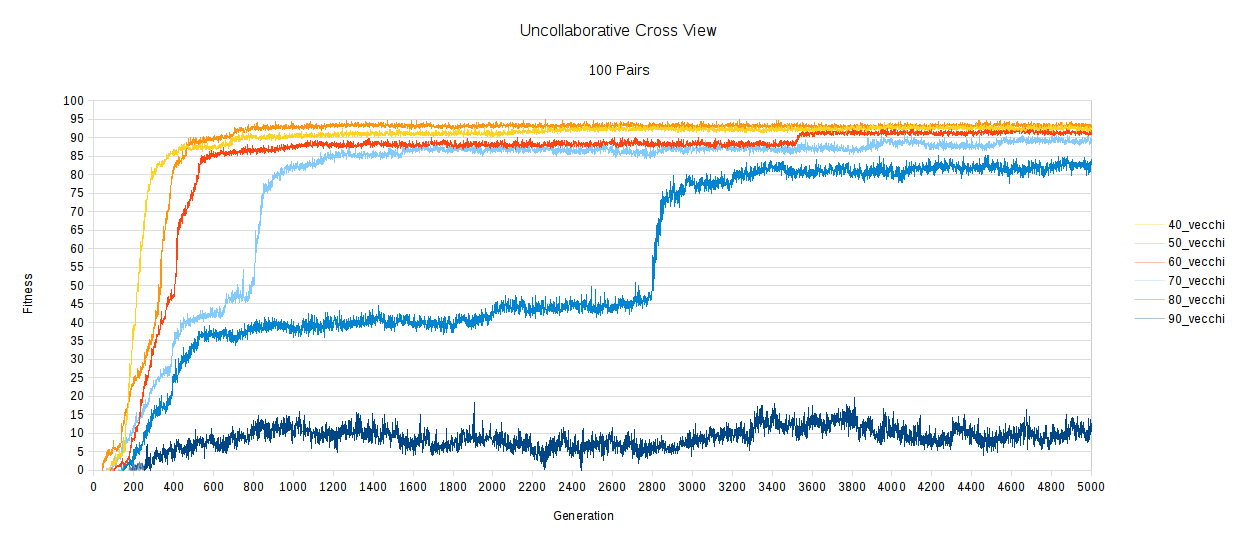
\includegraphics[scale=0.7,angle=90]{imgs/uncollaborative_cross_100_pairs_40_90_vecchi.png}
	\caption{Vista a croce non collaborativa, 100 coppie}
	\label{figure:uncoll_cross_100_40_90}
\end{figure}
\begin{figure}[ht]
	\centering
	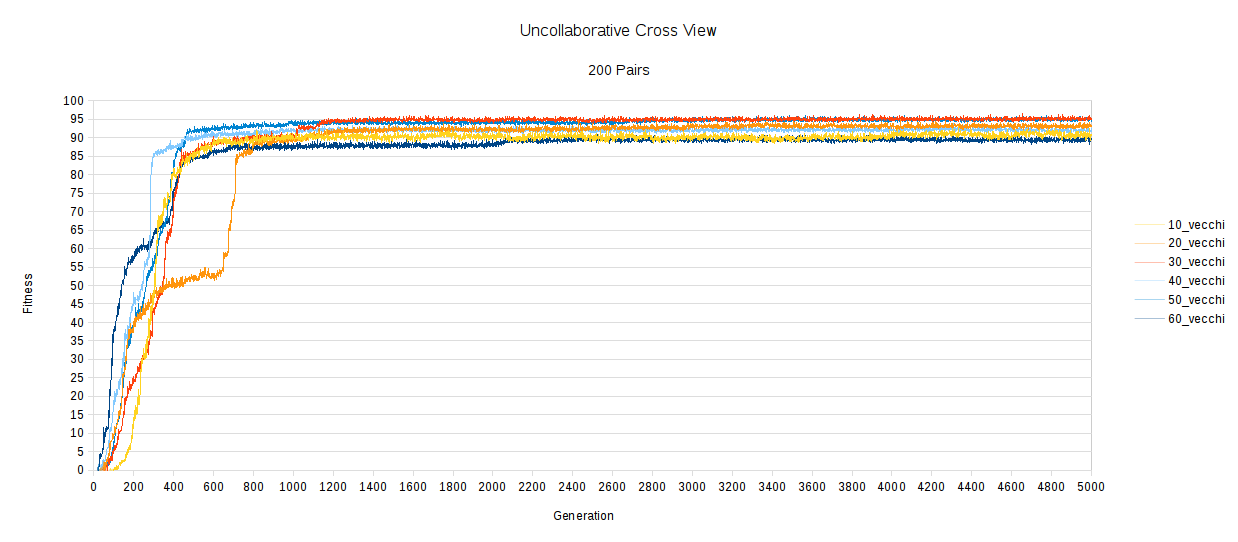
\includegraphics[scale=0.7,angle=90]{imgs/uncollaborative_cross_200_pairs_10_60_vecchi.png}
	\caption{Vista a croce non collaborativa, 200 coppie}
	\label{figure:uncoll_cross_200_10_60}
\end{figure}
\begin{figure}[ht]
	\centering
	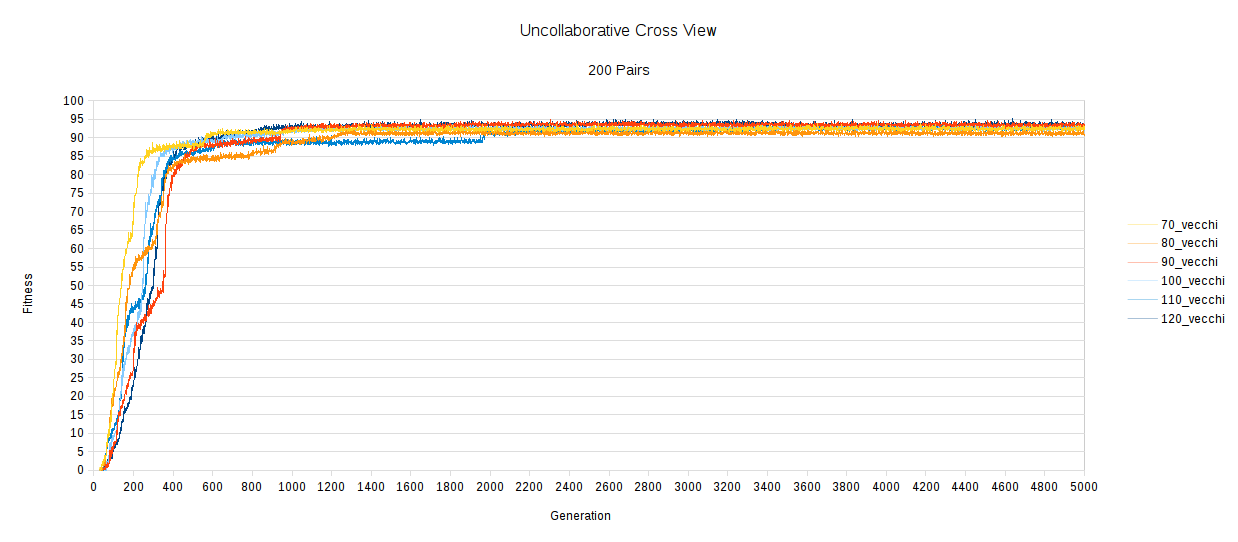
\includegraphics[scale=0.7,angle=90]{imgs/uncollaborative_cross_200_pairs_70_120_vecchi.png}
	\caption{Vista a croce non collaborativa, 200 coppie}
	\label{figure:uncoll_cross_200_70_120}
\end{figure}
\begin{figure}[ht]
	\centering
	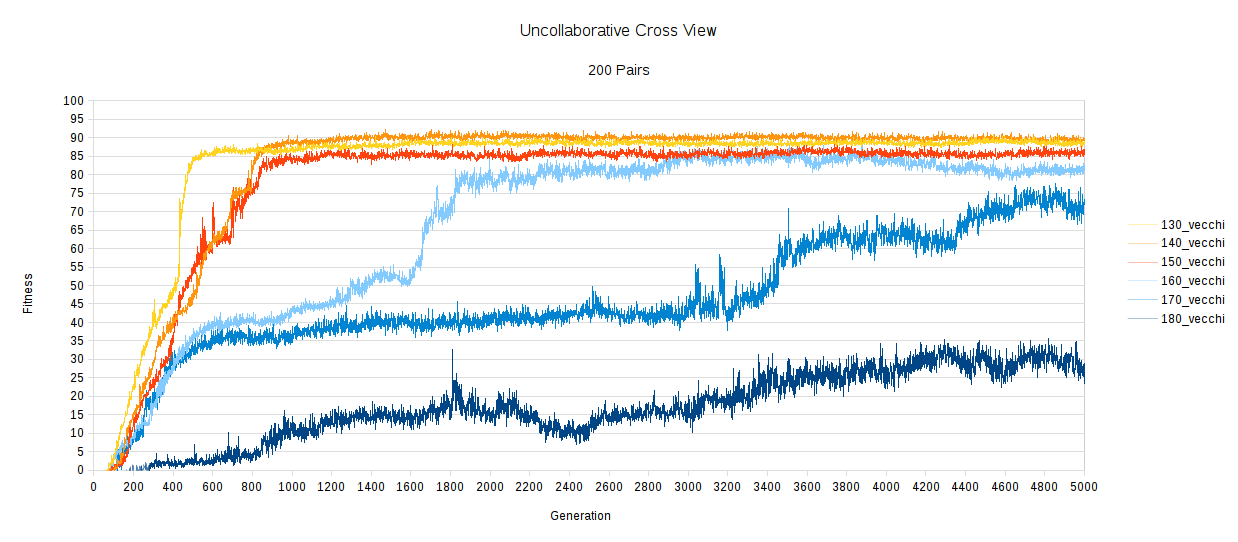
\includegraphics[scale=0.7,angle=90]{imgs/uncollaborative_cross_200_pairs_130_180_vecchi.png}
	\caption{Vista a croce non collaborativa, 200 coppie}
	\label{figure:uncoll_cross_200_130_180}
\end{figure}
\begin{figure}[ht]
	\centering
	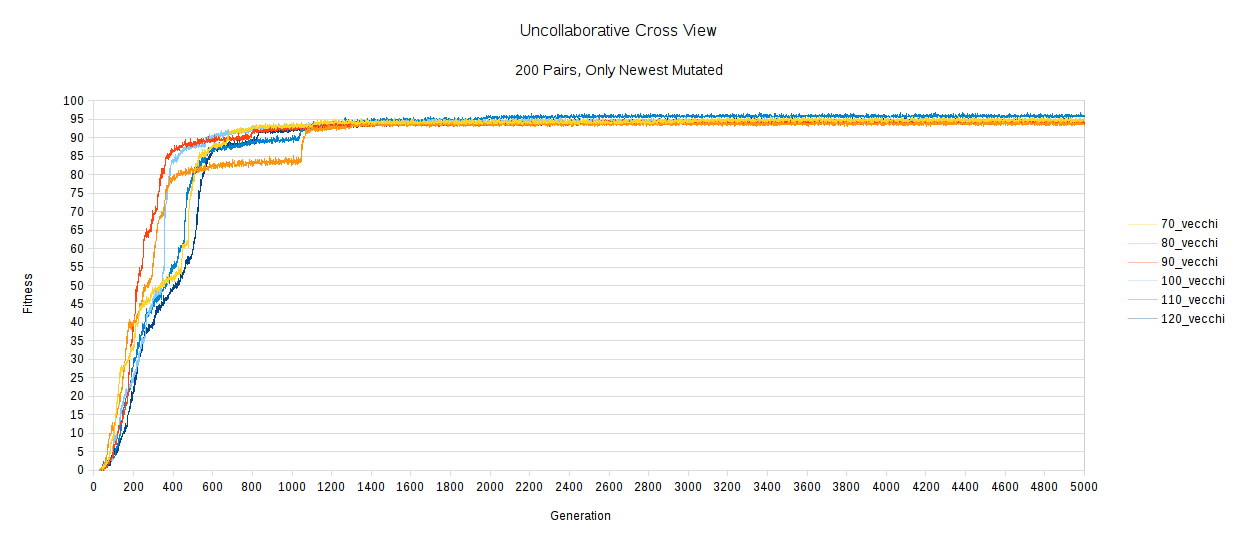
\includegraphics[scale=0.7,angle=90]{imgs/uncollaborative_cross_200_pairs_70_120_vecchi_solo_nuovi_mutati.png}
	\caption{Vista a croce non collaborativa, 200 coppie}
	\label{figure:uncoll_cross_200_70_120_vecchi_non_mutati}
\end{figure}
La prima simulazione è stata effettuata usando lo schema del paper con 100
coppie, ovvero 200 robot. In 5000 generazioni il valore di fitness, dopo un
primo incremento, si è sempre mantenuto attorno al valore 0. Questo ci ha fatto
supporre che la strategia di evoluzione da noi adottata potesse essere errata.
Abbiamo dunque deciso di copiare alcuni degli individui vecchi nella nuova
generazione.\newline
La Figura~\ref{figure:uncoll_cross_100_0_5} mostra i valori di 6 simulazioni
nelle quali abbiamo mantenuto da 0 a 5 coppie (le migliori) dalla vecchia alla
nuova generazione. Come è possibile notare, più sono gli individui che sono
mantenuti invariati e più alto è il valore di fitness raggiunto.\newline
In Figura~\ref{figure:uncoll_cross_100_10_35} abbiamo proseguito con il
ragionamento, copiando nella vecchia generazione da 10 a 35 coppie,
incrementando l'intervallo da 1 a 5. I valori di fitness si mantengono tutti fra
i 90 ed i 95 punti.\newline
A questo punto ci siamo chiesti quando le performance sarebbero crollate ed
abbiamo ulteriormente iterato il procedimento mantenendo da 40 a 90 coppie,
procedendo per intervalli di 10. Come è mostarto in Figura
\ref{figure:uncoll_cross_100_40_90}, man mano che il numero di coppie vecchie è
passato nella nuova generazione, il valore di fitness inizia a scendere, fino
a mostrare cali vertiginosi con 80 e 90 coppie.\newline
Avendo notato come la modifica anche piccola di un semplice parametro (il numero
di coppie vecchie da mantenere nella nuova popolazione) possa influenzare in
maniera significativa l'evoluzione, abbiamo deciso di ripetere lo stesso
procedimento aumentando il numero di coppie da 100 a 200. La Figura
\ref{figure:uncoll_cross_200_10_60} mostra l'andamento dell'evoluzione tenendo
da 10 a 60 coppie, la Figura~\ref{figure:uncoll_cross_200_70_120} da 70 a 120 e,
infine, la Figura~\ref{figure:uncoll_cross_200_130_180} grafica l'andamento dei
valori di fitness tenendo da 130 a 180 coppie.\newline
La differenza fra i valori di fitness raggiunti con 200 coppie rispetto ai
valori raggiunti con 100 coppie non è poi così grande. È però presente una
costante: i valori di fitness più alti sono raggiunti mantenendo una percentuale
di coppie vecchie da una generazione all'altra che va dal 10\% al 60\%.\newline
Abbiamo poi effettuato un'ultima simulazione tenendo i risultati migliori con
200 coppie dove le mutazioni genetiche sono state applicate solo ai nuovi
individui generati e non più anche ai vecchi. I risultati sono riportati in
Figura~\ref{figure:uncoll_cross_200_70_120_vecchi_non_mutati}.

\chapter{Conclusioni}
Come abbiamo visto nel capitolo precedente, lasciare agire due robot su una
mappa di 10x10 caselle nella quale sono state sparse 10 lattine, permette di
ottenere ottimi risultati, con un punteggio medio di fitness pari a 95 su 200
diverse sessioni. Questo significa, in media, raccogliere tutte e 10 le lattine
nella metà dei casi e 9 nell'altra.\newline
Abbiamo poi visto come la strategia evolutiva migliore sia quella élitaria,
ovvero, permettere ad un certo numero di robot di passare da una generazione
all'altra e come, non mutando questi individui, siano raggiunti valori ancora
migliori. La percentuale di coppie da lasciare invariata da una generazione alla
successiva è stata poi stimata fra il 10\% ed il 60\%, valori confermati su
popolazioni di 100 e 200 individui.\newline
Usare una popolazione più grande non consente di ottenere, con questa strategia
evolutiva, grossi miglioramenti, se non il raggiungimento dei valori di
fitness più grandi impiegando un numero di passi minore, grazie ad una varietà
genica maggiore.\newline
Usare una vista più grande, per quanto riguarda la non collaborazione (ovvero
impedendo ai robot di vedersi sulla mappa), non ha portato i robot né a
raccogliere in media più lattine, quindi a totalizzare un punteggio di fitness
maggiore, né a raccogliere lattine più velocemente, almeno per quanto riguarda
il lasciarli agire per un numero di passi pari al 30\% ed al 40\% di quelli
necessari ad esplorare tutta la mappa: 10x10 = 100 caselle, ovvero 30 e 40
passi.\newline
Infine, lasciare che i robot possano vedersi sulla mappa ha evidenziato, almeno
per quanto riguarda la strategia evolutiva da noi individuata, come questo possa
rivelarsi un fattore che ostacola l'azione dei due.\newline
Occore in ultima analisi sottolineare come, variando anche in piccola parte
alcuni dei parametri che regolano l'evoluzione, questo porti a grossi
cambiamenti nell'apprendimento dei robot. È dunque possibile che possano
esistere combinazioni di valori che portino anche le coppie che usano viste
``collaborative'' ad ottenere risultati migliori. Ad oggi, però, non siamo
ancora stati in grado di trovarli, o meglio, variare anche la percentuale di
mutazione sembra non essere la strada giusta.



\section{Sviluppi Futuri}
Lasciamo come sviluppi futuri la possibilità di ricercare nuove strategie
evolutive che permettano, se esistono, di evolvere i robot che usano viste
collaborative in modo da ottenere valori di fitness maggiori.\newline
Interessante sarebbe anche introdurre nuove strategie di cooperazione. Con
questo lavoro, infatti, ci siamo solamente dedicati a gettare le basi nello
studio di come possano più entità collaborare nell'azione comune su una mappa.
Abbiamo infatti analizzato le performance di un caso base, quello che usa una
vista a croce nella quale la possibilità di vedere gli altri robot non esiste,
in relazione all'uso di una vista nella quale i due Robby possono vedersi. Ciò
non vieta l'implementazione di ulteriori meccanismi di collaborazione, magari
più complessi, che vedano ad esempio lo scambio di informazioni tra le varie
entità, come la posizione assoluta o relativa nella mappa, o di scambiarsi la
vista, e così via\dots Ci teniamo comunque a sottolineare come l'azione
indpendente di due robot consente di raggiungere ottimi risultati (95 punti
fitess su 100 disponibili), il ché fissa un livello da superare molto alto per
eventuali strategie evolutive.\newline
Infine, comunichiamo ad eventuali interessati che il nostro codice
\cite{biblio:git} lascia la possibilità di usare anche una vista quadrata
collaborativa, da noi non usata per le varie prove. Potrebbe essere interessante
analizzare se l'uso di tale vista replichi i risultati ottenuti nella non
collaborazione, ovvero, dove usare una vista più grande non da alcun vantaggio.

\begin{thebibliography}{1}
	
	\bibitem{biblio:robby}
	Melanie Mitchell,\newline
	``\textit{Robby, The Soda-Can-Collecting Robot}''.\newline
	\url{http://web.cecs.pdx.edu/~mm/ArtificialIntelligenceFall2008/Homework/Homework6.pdf}.
	
\end{thebibliography}


\end{document}
